\section{SAM-Flow: From Native Gains to Equal Editing Response}
\label{sec:sam}
This section reports the prespecified SAM analyses with masked-input (MI) LPIPS. The main paper uses the feature-map (FM) measure for both operators. At its default setting, spatial SAM-Flow reduces background LPIPS by 0.06496 relative to the same editor with uniform projection. Two constants calibrated on the native trajectory recover 81.7\% of that reduction (95\% CI 77.0--86.1\%), while reducing directional CLIP by 0.04054 relative to uniform. Across all five measured settings at matched directional CLIP, spatial SAM retains a background advantage of $\ScanSUMean$ [$\ScanSULo,\ScanSUHi$] on $\ScanSUValid$ sources with overlapping responses. These quantities compare a default configuration, a change to its projection, and an operating point selected for the same measured edit response.

\subsection{Sources, prompts and regional scores}
We sampled five PIE-Bench sources in each of ten editing categories. Within category the sampling key was the SHA-256 digest of \texttt{A-dose-lens-pilot-20261117-v1:} followed by the 12-digit source ID. Selection used the 700-entry benchmark and preceded outcome scoring. The 50 selected images share neither IDs nor decoded RGB images with the 40-source primary correction cohort. Two development IDs recur, one from each earlier pilot (Section~\ref{sec:development}). Sources with global edits remain in the sample. In category order 0--9, the counts with a nonempty preservation region are $4,5,5,5,4,4,5,5,4,1$. All 50 have an edit region.

The editor received the recorded source and target prompts with the benchmark's annotation brackets removed. Token selection used the text spans and, in 20 cases, manually supplied context tokens identifying the affected noun or phrase. The source and a FlowEdit scout supply attention maps. Benchmark evaluation masks enter scoring only. Two discrepancies surfaced in the visual audit. The raw instruction for 611000000001 refers to a raven, while its image and model prompts concern an otter and colored hearts. For 812000000002 the raw instruction places a house in front of the girl, while the target prompt places the girl in front of a house. We retained both original model inputs and both sources throughout the prespecified analysis.

Given the binary edit mask $M_{\rm edit}$ on the $512\times512$ grid, the preservation mask is $B=1-M_{\rm edit}$. We multiply both RGB images in $[0,1]$ by $B$, convert to $[-1,1]$, and evaluate the learned AlexNet-v0.1 LPIPS scalar on the resulting full images. Black pixels replace the edit region before feature extraction. The scalar uses the network's spatial averaging without division by background area. The separate source-correction study weights an LPIPS \emph{distance map} computed on intact images. We compare LPIPS differences within the corresponding study.

Directional CLIP is the cosine between the change in unit-normalized CLIP ViT-B/32 image embeddings (output minus source) and the change in unit-normalized text embeddings (target minus source prompt). The image processor uses its 224-pixel input. A zero-norm embedding difference has undefined cosine. Edit-region MAE is the sum of RGB absolute differences in $[0,1]$ over $M_{\rm edit}$ divided by three times its pixel count. Empty support has a missing regional score. Background summaries therefore use 42 sources, and directional CLIP and edit-region MAE use all 50. Every output contributes to each score for which it has support. MAE quantifies change in the edit region, including changes to the wrong object.

\subsection{Projection, allocation and the two constants}
The published FLUX implementation of SAM-Flow~\cite{cui2026sam} is pinned to commit \path{8167978666e6df11e987a453934b89ec422bd3a4}. All arms share the FLUX.1-dev backbone, source, prompts, resolution, and generation seed 0 within source. The runner resets the generation seed for the shared scout and before each editing arm, pairing the draws for latent sampling and forward noise across the compared configurations. A separate seed, 999, controls the attention-reference noise. All five settings use the same generation seed on each source. The grid has 28 steps, SAM uses 26 active steps and eight noise averages. Its source/target guidance scales are 1.5/10.5. The independent FlowEdit reference~\cite{kulikov2025flowedit} uses its native differential update with target guidance 5.5 and default $n_{\max}=24$.

Let $A$ be the source anchor and $R_i=z_i^{\rm full}-A$ the accumulated proposed displacement. The model and visible states receive $A+P_i^k\odot R_i$, for branch $k=m,v$. With projection scale $\alpha$, native soft and hard gates $W_s,W_h$, core weight $C$, and ring-only weight $J$, the implemented factors are
\begin{align}
P_i^m &= \alpha W_s, &
P_i^v &= \alpha(CW_s+0.35\,J W_h).
\end{align}
The visible branch uses the original core/ring blending order. Uniform uses the same scalar at every location in both branches. Both arms retain the scout and prompt processing. Define $b_i^k=\RMS(P_i^k\odot R_i)$ over all latent coordinates. These are displacements after the Euler update, with the 26 active steps weighted equally. For the older velocity correction we integrate RMS with the step size $h_i$. Stronger projection here permits greater departure from the source. Stronger additive protection in the correction editor pushes the state toward the source.

For each source the constant comparator computes $p_k=\sum_i b_i^k/\sum_i\RMS(R_i)$ on the native spatial trajectory. It then applies $p_k$ at every location and step in its own rollout. The two fitted constants depend only on the reference profile. On the resulting trajectory the summed FP32 projection magnitude exceeds native by 8.42\% on average.

\begin{table}[!t]
\centering\footnotesize
\caption{SAM controls and the FlowEdit reference on 50 sources. Background LPIPS uses the original masked-input (MI) score on the 42 with a preservation region. $S$ and $U$ denote the native spatial and uniform profile origins.}
\label{tab:sam-core}
\begin{tabular}{@{}lrrr@{}}\toprule
Configuration & BG LPIPS & Dir.\ CLIP & Edit MAE\\\midrule
FlowEdit 24 & .1185 & .0842 & .0861\\
Native spatial & .0297 & .0841 & .0587\\
Uniform & .0947 & .0927 & .0863\\
Two constants & .0416 & .0521 & .0493\\
Uniform at $S$ & .0423 & .0546 & .0490\\
Spatial at $U$ & .0552 & .1100 & .0997\\\bottomrule
\end{tabular}
\end{table}
The recovery fraction is the ratio of two paired cohort-mean gains, $0.05310/0.06496$. Core uncertainty uses 20,000 paired source bootstrap draws (seed 20261118), recomputing the ratio in each draw. Relative to uniform, the two constants change directional CLIP by $-0.04054$ [$-0.05709,-0.02526$]. Relative to the constants, native spatial improves background LPIPS by $0.01186$ [0.00803, 0.01628] and increases directional CLIP by $0.03194$ [0.01485, 0.05031]. The CLIP increase is $0.04007$ [0.02123, 0.06039] on the same 42 sources that contribute LPIPS.

\subsection{Three default examples selected by directional CLIP}
\label{sec:sam-ranked}
Figure~\ref{fig:sam-ranked} shows the three rank-selected cases (dog, bag and painting). The dog also appears in main Fig.~3(b). To select the rows post hoc, we ranked all 50 sources independently on two directional-CLIP differences: uniform minus two constants and native spatial minus two constants. On each axis we divided the zero-based rank by 49, assigning tied scores their average rank. For the favorable, typical and contrary rows, respectively, we selected the point at the smallest Euclidean distance from $(0.9,0.9)$, $(0.5,0.5)$ and $(0.1,0.1)$. The favorable row required both differences to be positive and the contrary row required both to be negative. The typical row used all 50 sources. Equal distances were resolved by the lowest source ID.

For the dog (211000000000), the two directional-CLIP differences are $+0.1402$ and $+0.0888$, in uniform, then native spatial order. Both favor the corresponding default over the two-constant control. For the bag (524000000004) the differences are $+0.0190$ and $+0.0328$, yet all three outputs leave the bag upright. For the abstract-to-digital painting (000000000103), the differences are $-0.0122$ and $-0.0314$. Here the two-constant control has the highest directional CLIP.

\begin{figure*}[!t]
\centering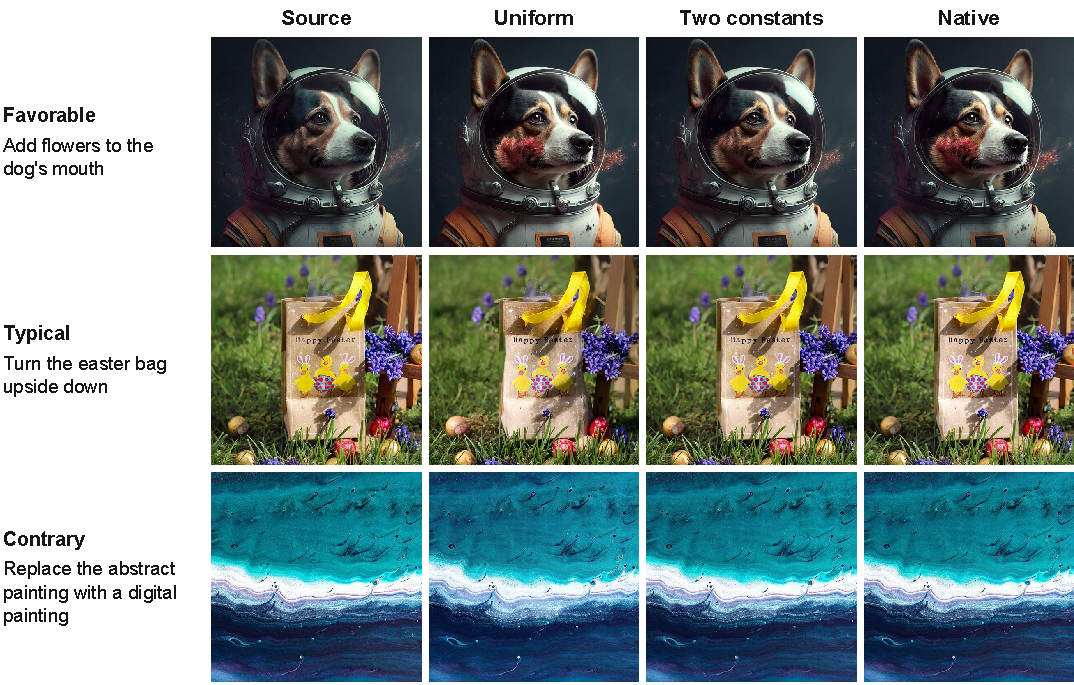
\includegraphics[width=\textwidth]{supp_sam_examples.pdf}
\caption{Three default SAM-Flow comparisons selected by the joint ranks of two directional-CLIP contrasts. Each row pairs the source with the uniform, two-constant and native spatial outputs at seed 0. All four views retain the full $512\times512$ field. The high-ranked dog shows color beside its muzzle; flowers held in its mouth are difficult to discern, the typical bag remains upright, and the contrary painting yields a higher text-response score under two constants than under either other setting.}
\label{fig:sam-ranked}
\end{figure*}

\subsection{Crossing the two measured projection profiles}
At every active step, replay recomputes the candidate direction on its own state and scales its RMS to the prescribed branch target. A zero target returns zero displacement. A positive target requires a nonzero candidate norm. At the spatial-origin profile, spatial minus uniform changes masked-input background LPIPS (MI) by $-0.01258$ [$-0.01673,-0.00894$] and directional CLIP by $+0.02947$ [0.01172, 0.04866]. At the uniform origin these contrasts are $-0.03950$ [$-0.05064,-0.02950$] and $+0.01738$ [$-0.00458,0.03979$]. The latter CLIP contrast on the 42 preservation-eligible sources is $+0.02485$ [0.00048, 0.04956].

The four MI-LPIPS cells yield two paths through the same native difference. Changing allocation at the spatial origin contributes $-0.01258$, and changing profile along the uniform allocation contributes $-0.05238$. Changing profile along the spatial allocation contributes $-0.02545$, and changing allocation at the uniform origin contributes $-0.03950$. Both paths give $-0.064957$ to six decimals when computed from unrounded cells. The post hoc CPR interaction in MI-LPIPS (allocation contrast at $S$ minus that at $U$) is $+0.02693$ [0.01856, 0.03631], positive on 41/42 sources (20,000 paired source resamples, seed 1208). The two historical source-correction paths appear in Table~\ref{tab:paths}.

Both branches at all 26 steps pass the pre-cast FP32 tolerance $10^{-6}+10^{-4}b_i^k$ in 100/100 replay runs. Comparing realized source-relative BF16 states after casting, with tolerance $10^{-6}+0.01b_i^k$, gives all-step passes in 3/50 uniform-at-spatial and 34/50 spatial-at-uniform runs. The largest single-step relative error is 11.39\%. The largest source/branch sum of absolute errors divided by the sum of its target RMS values is 0.336\%.

Replaying a target can take a blend outside the native convex range. We measured the effective coefficient as replay gain times the native factor at each location for spatial allocation, and as the gain itself for uniform allocation. At least one coefficient exceeded $1+10^{-6}$ in both branches of all 50 spatial-at-uniform runs (model maximum 2.04984, visible maximum 4.73960). Under uniform-at-spatial, 2/50 model branches exceeded the threshold (maximum 1.00847) and 0/50 visible branches did (maximum 0.95588). Replay retains these coefficients to prescribe the requested magnitude. At the measured scale $\alpha=1.25$, all 50 sources reached effective factors above one on both branches of both scanned arms, at each of the 26 active steps. For spatial gates the exceedance is a maximum over locations. The four scales through the default $\alpha=1$ stayed within the convex range. The archive provides per-source extrema in \path{analysis/v21_bounded/gate_ranges.csv}.

\subsection{Response-matched scan and coverage}
\label{sec:sam-scan}
Each source has five settings per arm. Native spatial varies its scale and uniform varies its uniform factor over $\{0.25,0.5,0.75,1,1.25\}$. FlowEdit varies $n_{\max}$ over $\{12,16,20,24,28\}$. The 750 curve points include 150 reused defaults and 600 additional outputs. The three remaining core controls contribute 150 distinct outputs, bringing the archive to 900/900 completed jobs. Figure~\ref{fig:sam-scan}(A) follows the response of each source across the five settings. Table~\ref{tab:sam-points} summarizes each setting across sources.

\begin{table}[!t]
\centering\scriptsize\setlength{\tabcolsep}{2.7pt}
\caption{Five settings per arm. Background LPIPS uses masked inputs (MI). Each row summarizes the observed images at one setting. Stars mark the three defaults.}
\label{tab:sam-points}
\begin{tabular}{@{}lrrrrrr@{}}\toprule
 & &\multicolumn{3}{c}{Directional CLIP}&\multicolumn{2}{c}{BG LPIPS}\\
Arm & Knob & $n$ & Mean & Median & $n$ & Mean\\\midrule
\ScanPointRows
\bottomrule\end{tabular}
\end{table}

For each source and arm, connect adjacent observed $(x,L)$ pairs in increasing knob order, where $x$ is directional CLIP and $L$ is preservation LPIPS. At a response with several crossings, take the earliest segment in knob order. For a vertical segment use the first endpoint. Each comparison requires all five finite pairs in both arms. Its lower endpoint $a$ is the larger of the two minimum responses, and $b$ is the smaller maximum. A separated range ($b<a$) or a single point ($b=a$) contributes to coverage only. When $b>a$, evaluate
\begin{equation}
d_j=(b-a)^{-1}\int_a^b [L_{\rm first\ arm}(x)-L_{\rm second\ arm}(x)]\,dx .
\end{equation}
Split the interval at all response knots in either curve. Midpoint evaluation on each subinterval integrates the selected affine branches exactly. Each valid source receives equal weight regardless of its interval width. We bootstrap the mean of these paired differences 10,000 times, resampling valid sources with replacement in ascending-ID order (PCG64, seed 0 restarted for each pair, linear percentile endpoints). The intervals are conditional on observed common support.

\begin{figure*}[!t]
\centering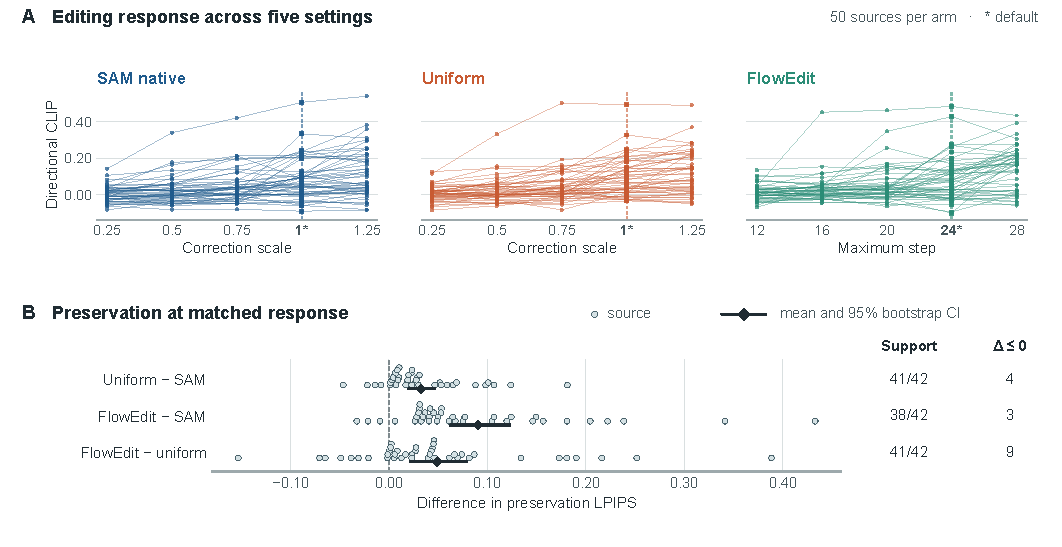
\includegraphics[width=\textwidth]{figures/scan_profile.pdf}
\caption{Five measured settings and paired masked-input background LPIPS (MI) at equal directional CLIP. (A) Each line follows one of 50 sources in knob order. The SAM scale sets the native spatial projection strength or the uniform projection factor. FlowEdit varies its maximum step. Stars mark the defaults. (B) Each dot is one source's interval-average background LPIPS difference over its pair's shared response range. Diamonds give equal-source means and bars show 95\% paired bootstrap intervals. A positive value favors the second named arm. Support is the number with positive-width overlap among the 42 sources with a background. The last column counts nonpositive differences.}
\label{fig:sam-scan}
\end{figure*}

\begin{table*}[!t]
\centering\small
\caption{Prespecified first-crossing analysis. ``Missing/disjoint/touch'' counts are among the 42 preservation-eligible sources. Width is median common directional-CLIP width. Differences are in background LPIPS. Positive favors the second named arm.}
\label{tab:sam-support}
\begin{tabular}{@{}lcrrrrrr@{}}\toprule
Contrast & Valid/eligible & Missing/disjoint/touch & Width & Mean & 95\% CI & Median & $d_j\leq0$\\\midrule
\ScanPairRows
\bottomrule\end{tabular}
\end{table*}
In Fig.~\ref{fig:sam-scan}(B) and Table~\ref{tab:sam-support}, the primary contrast is uniform minus native spatial. $\ScanSUPositive$ of $\ScanSUValid$ source differences are positive, four are negative, and source 712000000004 has disjoint response ranges. At the defaults, the mean difference on those same 41 sources is 0.0658. For the two secondary comparisons, FlowEdit minus spatial is positive on 35/38 sources and FlowEdit minus uniform on 32/41. Each comparison uses its own common response range and source set.

\subsection{Sensitivity and held-out prediction}
Switching to the last crossing changes the primary mean to $+0.03812$ [0.02431, 0.05300] (35 positive, 41 valid). Using edit-region MAE as the response gives $+0.03619$ [0.02420, 0.04959] (36 positive, 42 valid, median common width 0.07834 MAE). Excluding the two prompt discrepancies identified in the atlas gives $+0.03223$ [0.01918, 0.04671] with 35 positive among 39 overlapping sources (48 retained, 40 preservation-eligible, one disjoint). These are post hoc changes to the response definition, crossing convention or sample. The primary result retains both flagged sources and uses first crossing at equal directional CLIP.

A separate post hoc prediction targets the default background LPIPS reduction, uniform minus spatial. For each of the 42 eligible sources we fit ordinary least squares on the other 41. An intercept alone yields held-out RMSE/MAE 0.05104/0.03975. Background area fraction gives 0.05011/0.03930. Adding $1-\bar b^v_S/\bar b^v_U$, the relative attenuation in mean visible projected RMS across the two default rollouts, gives 0.04630/0.03401. The extra predictor thus uses information from running both default configurations on the held-out image. The validation population is the SAM cohort.

\subsection{Recorded execution cost}
A single RTX 4080 SUPER ran BF16 inference with model CPU offload (PyTorch 2.8.0+cu128, Diffusers 0.35.1, Transformers 4.56.2). The 300 core scientific jobs sum to 12.38 hours and 125,468 transformer evaluations. A resumed run reused 245 completed jobs and finished 55. The 600 additional scientific jobs sum to 22.52 hours and 229,800 evaluations: 200 native jobs took 9.43 hours/85,800 evaluations, 200 uniform jobs took 7.42 hours/83,200 evaluations, and 200 FlowEdit jobs took 5.67 hours/60,800 evaluations. Total recorded job time is 34.89 hours with 355,268 evaluations. Job times exclude failed launches, engineering checks, idle intervals and separate metric evaluation.
